%------------------------ Packages ------------------------
\documentclass[12pt,a4paper]{article}
\usepackage[latin1]{inputenc}
\usepackage[T1]{fontenc}
\usepackage[pdftex]{graphicx}
\usepackage{float}
\usepackage{amsmath}
\usepackage{amssymb}
\usepackage[FIGTOPCAP]{subfigure}
\usepackage{color}
\usepackage[hidelinks]{hyperref}

\newcommand{\version}{\IfFileExists{../../version.txt}
{\input{../../version.txt}}
{\input{../../../version.txt}}
}

\newcommand{\command}[1]{%
\indent \fcolorbox{black}{white}{%
   \begin{minipage}{\dimexpr\textwidth-\parindent\relax}%
      #1
   \end{minipage}%
}
}

\newsavebox{\FVerbBox}
\newenvironment{sample}
{\par \vspace{0.2cm} \begin{lrbox}{\FVerbBox}
\begin{minipage}{\dimexpr\textwidth-\parindent\relax}}
{\end{minipage}
\end{lrbox}
\fcolorbox{black}{lightgray}{\usebox{\FVerbBox}}
\vspace{0.2cm}}

\newenvironment{sampletitle}
{\vspace{0.2cm} \noindent\textbf{Example} :
\begin{sample}}
{\end{sample}}

\newcommand{\samplecomment}[1]{%

\textit{#1}
}

\newcommand{\seealso}[1]{\vspace{0.2cm} \noindent\textbf{See also} :\par #1}

% tikz
\usetikzlibrary{calc}
\usetikzlibrary{arrows}
\usetikzlibrary{shadows}

\tikzset{block/.style={draw, text centered, fill=gray!10,drop shadow}}
\tikzset{connect/.style={draw, line width=1 pt}}

\begin{document}

\begin{center}
\textbf{\huge  \underline{Sobel operator}}
\end{center}
\vspace{0.5cm}

Sobel operator 3 * 3 use ..... brief

\begin{figure}[h!]
\centering
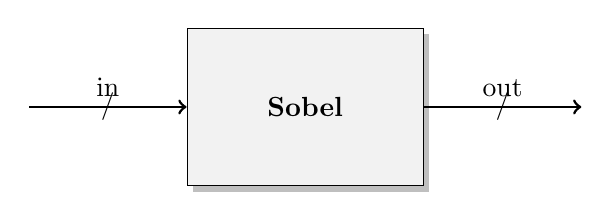
\begin{tikzpicture}
\node[block,rectangle,minimum height=2cm,minimum width=3cm] (bloc) {\textbf{Sobel}};

\path[connect,<-] ([yshift=0.0cm]bloc.west) -- node{/} node[above]{in} ++(-2cm,0);

\path[connect,->] ([yshift=0.0cm]bloc.east) -- node{/} node[above]{out} ++(2cm,0);
 ([xshift=0.5cm,yshift=-0.6cm]bloc.north);

\end{tikzpicture}
\end{figure}

\begin{figure}[!h]
\centering
\subfigure[Initial image]{
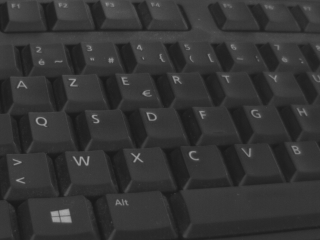
\includegraphics[width=5cm]{sobel1.png}}
\hspace{2cm}
\subfigure[Image with Sobel operator]{
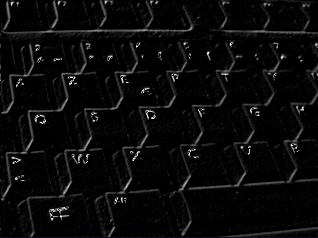
\includegraphics[width=5cm]{sobel2.png}}
\end{figure}

\section*{Properties}
\properties{
enable & bool & Enable the processing \\ 
}

\section*{Constants}

\section*{Equivalence}
\subsection*{Matlab}

\lstset{language=Matlab}
\begin{lstlisting}
%% Matlab - Sobel edge detection

I = imread('cell.tif');
figure, imshow(I), title('Original image');
SOBEL = edge(I, 'sobel');
figure, imshow(SOBEL)

\end{lstlisting}


\subsection*{OpenCV}

\lstset{language=C++}
\begin{lstlisting}
/// OpenCV - Sobel edge detection

/// Gradient X
  Sobel( src_gray, grad_x, ddepth, 1, 0, 3, scale, delta, BORDER_DEFAULT );
  convertScaleAbs( grad_x, abs_grad_x );

/// Gradient Y
  Sobel( src_gray, grad_y, ddepth, 0, 1, 3, scale, delta, BORDER_DEFAULT );
  convertScaleAbs( grad_y, abs_grad_y );

/// Total Gradient (approximate)
  addWeighted( abs_grad_x, 0.5, abs_grad_y, 0.5, 0, grad );

\end{lstlisting}

\section*{Mathematical formalism}

The operator uses 2 $3x3$ kernels which are convolved with the original image to compute approximations of the horizontal and vertical derivatives. \\

If we define $I$ as the source image, $\bigtriangledown_x$ and $\bigtriangledown_y$ as the horizontal and vertical derivative approximation respectively. $\bigtriangledown_x$ and $\bigtriangledown_y$ are written as follows :\\

\begin{equation}\label{eq1}
\bigtriangledown_x = \begin{pmatrix}
-1 & 0 & 1 \\ 
-2 & 0 & 2 \\ 
-1 & 0 & 1
\end{pmatrix}*I
\end{equation}

\vspace{0.5cm}

\begin{equation}\label{eq2}
\bigtriangledown_y = \begin{pmatrix}
-1 & -2 & -1 \\ 
0 & 0 & 0 \\ 
1 & 2 & 1
\end{pmatrix}*I
\end{equation}

\vspace{0.5cm}

We can develop (\ref{eq1}) and (\ref{eq2}) as follows :\\

\begin{equation}\label{eq3}
\begin{matrix}
\bigtriangledown_x = \begin{pmatrix}
-1 & 0 & 1 \\ 
-2 & 0 & 2 \\ 
-1 & 0 & 1
\end{pmatrix}*I  = \begin{pmatrix}
-1 & 0 & 1 \\ 
-2 & 0 & 2 \\ 
-1 & 0 & 1
\end{pmatrix}* \begin{pmatrix}
i_{00} & i_{01} & i_{02} \\ 
i_{10} & i_{11} & i_{12}\\ 
i_{20} & i_{21} & i_{22}
\end{pmatrix}  \\ 
& & \\
 =  -i_{00}-2i_{10}-i_{20}+i_{02}+2i_{12}+i_{22} \\ 
\end{matrix}
\end{equation}

\vspace{1cm}

\begin{equation}\label{eq4}
\begin{matrix}
\bigtriangledown_y = \begin{pmatrix}
-1 & -2 & -1 \\ 
0 & 0 & 0 \\ 
1 & 2 & 1
\end{pmatrix}*I  = \begin{pmatrix}
-1 & -2 & -1 \\ 
0 & 0 & 0 \\ 
1 & 2 & 1
\end{pmatrix}* \begin{pmatrix}
i_{00} & i_{01} & i_{02} \\ 
i_{10} & i_{11} & i_{12}\\ 
i_{20} & i_{21} & i_{22}
\end{pmatrix}  \\ 
& & \\
 =  -i_{00}-2i_{01}-i_{02}+i_{20}+2i_{21}+i_{22} \\ 
\end{matrix}
\end{equation}
 
\vspace{0.5cm}

In each point, we give an approximation of the gradient norm by the equation (\ref{eq5})

\begin{equation}\label{eq5}
\bigtriangledown = \sqrt{\bigtriangledown_x^2 + \bigtriangledown_y^2 } \simeq \bigtriangledown_x + \bigtriangledown_y
\end{equation}

\vspace{0.5cm}

Thus, we obtain :

\begin{equation}\label{eq6}
\bigtriangledown \simeq 2(i_{12}+i_{22}+i_{21}-i_{00}-i_{10}-i_{01})
\end{equation}
 
\vspace{0.25cm}
 
And finally in matrix form : 

\begin{equation}\label{eq7}
\kappa_S  \simeq \begin{pmatrix}
-2 & -2 & 0\\ 
-2 & 0 & 2\\ 
 0 & 2 & 2
\end{pmatrix}
\end{equation}

\end{document}